% revisar que haya referencias en todas las secciones

\documentclass[11pt,onecolumn]{article}
\setlength{\columnsep}{0.5cm}

\usepackage[utf8]{inputenc}
\usepackage[T1]{fontenc}
\usepackage[spanish]{babel}
\usepackage{hyperref}
\usepackage{graphicx}
\usepackage{natbib}
\usepackage{rotating}

\title{\vspace{-15mm}%
	\fontsize{24pt}{10pt}\selectfont
	\textbf{Estado del arte de la investigación sobre wikis}
	}	
\author{%
	\large
	\textsc{Emilio J. Rodríguez-Posada} \\
	\normalsize	Universidad de Cádiz \\
	\normalsize	\href{mailto:emiliojose.rodriguez@uca.es}{emiliojose.rodriguez@uca.es}
	\vspace{-5mm}
	}
\date{}


\begin{document}

\maketitle

\begin{abstract}

\end{abstract}

\section{Introducción}

%En principio lo que voy a hacer es analizar el estado del arte de la investigación de wikis, contar WikiPapers, y un poco de mi trayectoria en estos temas, cuestiones abiertas, conclusiones y trabajo futuro.

%Quizás para que fuera abordable el estado del arte, podría limitarme a clasificar los papers del último o dos últimos WikiSym. Y al último PAN/CLEF, WikiAI, MathWikis, Wikimania, WikiViz, etc. Comentar la existencia de todos estos eventos.

%Reutilizar cosas que haya escrito ya en mis papers.

El interés de los investigadores por los wikis, en especial Wikipedia, ha ido en aumento en los últimos años. La primera edición de WikiSym, un simposio sobre wikis, se celebró en 2005 y desde entonces han aparecido multitud de congresos, \emph{workshops}, conferencias y competiciones en este área. El estudio de los wikis es un campo emergente y prolífico.

Ha habido varios intentos, aunque con escaso éxito, de recopilar toda la literatura sobre wikis. Unas veces el enfoque o la herramienta utilizada eran limitados, otras debido a las dimensiones de la tarea el proyecto era abandonado y al poco tiempo los metadatos bibliográficos se perdían. En este trabajo presentamos WikiPapers, un proyecto colaborativo para recopilar toda la literatura sobre wikis. Se hace uso de MediaWiki y su extensión semántica, ambos conocidos por los investigadores de este campo. Hasta noviembre de 2012 se han recopilado más de 1.700 publicaciones y sus metadatos, además de documentación sobre herramientas y \emph{datasets} relacionados. Los metadatos son exportables en los formatos BibTeX, RDF, CSV y JSON. Los historiales completos del wiki están disponibles para descargar y facilitar su preservación. El proyecto está abierto a la participación de todo el mundo.

El resto del trabajo se divide de la siguiente manera. En la sección~2 motivamos este trabajo haciendo un repaso a los distintos enfoques utilizados hasta ahora para recopilar toda la literatura sobre wikis, incidiendo en sus ventajas e inconvenientes. En la sección~3 detallamos los objetivos. En la sección~4 definimos algunos términos que servirán para comprender mejor el contenido. En la sección~5 presentamos WikiPapers, cómo funciona y qué pasos se han dado. En la sección~6 hacemos un estado del arte empleando WikiPapers. En la sección~7 repasamos las cuestiones que a día de hoy siguen abiertas o que han tenido poca atención hasta ahora. Finalmente, en la sección~8, terminamos con unas conclusiones y trabajo futuro.

\clearpage

\section{Motivación}

El interés de los investigadores por los wikis, en especial Wikipedia, ha ido en aumento en los últimos años (Figura~\ref{fig:wptimeline}). La primera edición de WikiSym, un simposio sobre wikis, se celebró en 2005 y desde entonces han aparecido multitud de congresos (CLEF/PAN Lab), \emph{workshops} (WikiAI, SemWiki y MathWikis), conferencias (Wikimania, WikiCon, SMWCon, Wiki Conference India, Wikipedia Academy y Wikipedia CPOV Conference) y competiciones (WikiViz). El estudio de los wikis es un campo emergente y prolífico. Ha habido varios intentos, aunque con escaso éxito, de recopilar toda la literatura sobre wikis ~\citep{ayers2011}. Unas veces el enfoque o la herramienta utilizada eran limitados, otras debido a las dimensiones de la tarea el proyecto era abandonado y al poco tiempo los metadatos bibliográficos se perdían. Se han hecho recopilaciones en páginas personajes y blogs, a través de revisiones de literatura, haciendo uso de gestores de bibliografía, en páginas de Wikipedia y también en servicios como Zotero o CiteULike. A continuación los describimos y evaluamos sus ventajas e inconvenientes y cómo WikiPapers resuelve las carencias de estos enfoques.

\begin{figure*}[htb]
    \centering
    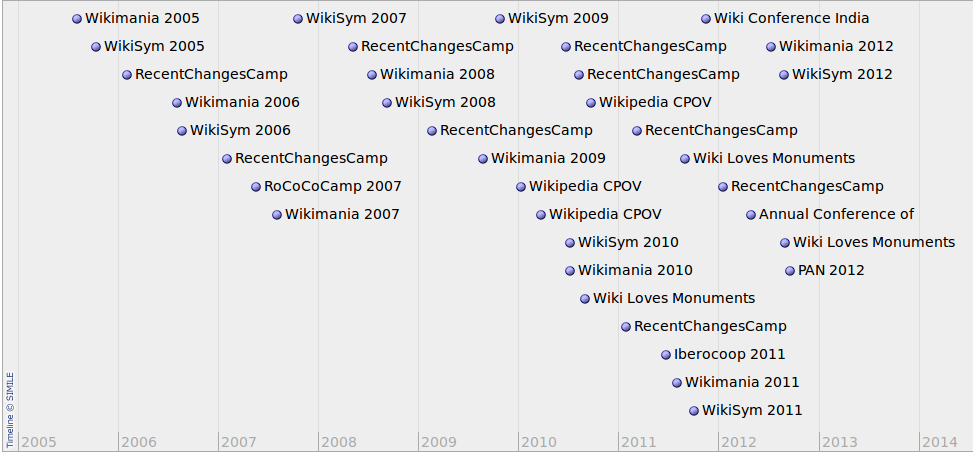
\includegraphics[width=\textwidth]{wptimeline.png} %two-column float
    \caption{Línea temporal de eventos sobre wikis.}
    \label{fig:wptimeline}
\end{figure*}

\subsection{Páginas personales y blogs}
Algunos autores han hecho recopilaciones de literatura en webs personales\footnote{\href{http://www.public.iastate.edu/~CYBERSTACKS/WikiBib.htm}{http://www.public.iastate.edu/~CYBERSTACKS/WikiBib.htm}} y blogs. Un ejemplo bastante completo de este último tipo es SWEETpedia,\footnote{\href{http://www.mkbergman.com/sweetpedia/}{http://www.mkbergman.com/sweetpedia/}} que contiene publicaciones sobre wikis y semántica. Uno de los inconvenientes de este sistema es que el esfuerzo suele recaer sobre una única persona y los metadatos no son fácilmente exportables. En WikiPapers el trabajo se hace colaborativamente y todos los metadatos son fácilmente exportables en diversos formatos.

\subsection{Gestores bibliográficos}

\subsubsection{En servidores propios}
Se han empleado gestores bibliográficos como WIKINDX\footnote{\href{http://sourceforge.net/projects/wikindx/}{http://sourceforge.net/projects/wikindx/}} creando portales propios como Wikibibliographie ENCYCLEN\footnote{\href{http://wikindx.inrp.fr/biblio_encyclen/}{http://wikindx.inrp.fr/biblio\_encyclen/}} y otros ya desaparecidos, pero como contrapartida decidieron restringir la edición a un círculo de usuarios aprobados. Sin embargo, en WikiPapers pueden participar tanto usuarios registrados como sin registrar.

%\href{http://toolserver.org/~voj/bibliography/}{http://toolserver.org/~voj/bibliography/}
%\href{http://wikiindex.org/Wiki_Research_Bibliography}{http://wikiindex.org/Wiki\_Research\_Bibliography}

\subsubsection{Servicios web y redes sociales}
Existen servicios web y redes sociales con recopilaciones de literatura sobre wikis, en Zotero,\footnote{\href{https://www.zotero.org/groups/wikipedia_research}{https://www.zotero.org/groups/wikipedia\_research}} BibSonomy\footnote{\href{http://www.bibsonomy.org/tag/wikipedia}{http://www.bibsonomy.org/tag/wikipedia}} \footnote{\href{http://www.bibsonomy.org/tag/wiki}{http://www.bibsonomy.org/tag/wiki}} y CiteULike.\footnote{\href{http://www.citeulike.org/tag/wikipedia}{http://www.citeulike.org/tag/wikipedia}}\footnote{\href{http://www.citeulike.org/tag/wiki}{http://www.citeulike.org/tag/wiki}}\footnote{\href{http://www.citeulike.org/group/382}{http://www.citeulike.org/group/382}} Este enfoque sí hace uso de una comunidad de usuarios para procesar las publicaciones, pero de nuevo requieren registrarse, y la capacidad de estos servicios para aprovechar los metadatos generando tablas o gráficos es inexistente.

\subsection{Buscadores}
Google Scholar,\footnote{\href{http://scholar.google.es}{http://scholar.google.es}} con buena cobertura, carece de representaciones visuales y no permite comentarios. Microsoft Academic Search\footnote{\href{http://academic.research.microsoft.com}{http://academic.research.microsoft.com}} es gráficamente muy bueno, pero excluye material relacionado como datasets o herramientas. La capacidad de dar contexto a las publicaciones en WikiPapers de forma manual no puede ser superada por un buscador
automático típico.

\subsection{Recopilaciones en Wikipedia}
También existen listados de publicaciones y recursos en algunas Wikipedias, como en la versión alemana\footnote{\href{http://de.wikipedia.org/wiki/Wikipedia:Wikipedistik/Bibliographie}{http://de.wikipedia.org/wiki/Wikipedia:Wikipedistik\\ /Bibliographie}} y la inglesa\footnote{\href{http://en.wikipedia.org/wiki/Wikipedia:Academic_studies_of_Wikipedia}{http://en.wikipedia.org/wiki/Wikipedia:Academic\\ \_studies\_of\_Wikipedia}}. El principal inconveniente de este enfoque es que no es posible jugar con los datos dentro del mismo wiki, al estar todo escrito como texto plano, sin enriquecimiento semántico. En WikiPapers todos los metadatos son propiedades semánticas, tanto en las llamadas \emph{infoboxes} (tablas) como en el cuerpo del artículo.

\subsection{Revisiones de literatura}
Finalmente, se han realizado varias revisiones de literatura con diferente grado de exhaustividad. La primera de ellas ~\citep{voss2005} se hizo en un momento en el que las publicaciones eran escasas, pero ya se podía ver una tendencia de publicación creciente y la presencia de muchas preguntas por responder. Un año más tarde ~\citep{ayers2006} vuelve a hacer un repaso a la literatura existente y enumera aquellas áreas que han recibido interés: historiales, páginas de discusión, contenido de los artículos, políticas del sitio, citas a artículos, encuestas a usuarios y listas de correo.

No sería hasta 3 años después cuando \cite{okoli2009b} presentan una propuesta de protocolo para hacer un mapeo sistemático de la literatura sobre Wikipedia, indicando la existencia de más de 1.000 publicaciones y ese mismo año \cite{okoli2009} analiza el estado del arte. Dos años más tarde, \cite{nielsen2011} hace la mayor revisión de literatura en un documento de más de 50 páginas, en progreso e inacabado, que incluye 300 referencias a publicaciones y reincide en la existencia de 1.000 publicaciones sobre el tema.

\cite{martin2011} hace primero un repaso técnico a la estructura de la base de datos (páginas, usuarios, texto), luego se centra en las áreas de calidad y acaba con unas consideraciones filosóficas.

\cite{okoli2012} hacen una revisión de la literatura y han creado un wiki reutilizando las plantillas, formularios, semántica y estructura de WikiPapers. Están trabajando en el análisis de un subconjunto de la literatura, en este caso la relativa a Wikipedia exclusivamente. Es un proyecto temporal y pretenden incorporar sus resultados a WikiPapers.

La revisión más reciente \cite{jullien2012} hace un repaso por las motivaciones para contribuir, roles, estructura, la vida de un artículo, calidad, experiencia de usuario y accesibilidad, entre otros.

Uno de los inconvenientes de estas revisiones de literatura es que quedan rápidamente desactualizadas debido al ritmo con el que aparecen nuevas publicaciones. WikiPapers es actualizado continuamente por su comunidad de voluntarios.

\clearpage

\section{Objetivos}

Los objetivos de este proyecto de investigación son:

\begin{enumerate}
\item Idear un sistema o adaptar alguno existente que permita recopilar literatura sobre wikis, superando las carencias de los enfoques usados anteriormente.
\item Deberá permitir añadir, eliminar y modificar metadatos bibliográficos fácilmente, de manera manual e importando en lotes.
\item Usará características de la web semántica para poder sacar el máximo provecho posible a los metadatos.
\item Se pondrá atención en que los datos sean leibles tanto por humanos como por máquinas.
\item Tendrá licencia libre (por tanto los contenidos serán reutilizables por terceros) y facilitará la exportación de los metadatos.
\item Realizar un estado del arte haciendo uso del sistema creado en los puntos anteriores y con las publicaciones que se hayan podido recopilar hasta el momento. No será exhaustivo pero sí incluirá lo más relevante, ya que el propio proyecto es un estado del arte vivo que es continuamente actualizado.
\end{enumerate}

\clearpage

\section{Definiciones, acrónimos y abreviaturas}

%Mirar las que definí en mi PFC y meter otras más nuevas

A continuación se incluyen algunas \textbf{definiciones, acrónimos y abreviaturas} que facilitan la comprensión de este trabajo.

\textbf{Administrador}: Persona que se dedica al mantenimiento de un sistema o red. En Wikipedia hace referencia a aquellos usuarios que pueden borrar/restaurar páginas, bloquear/desbloquear usuarios y proteger/desproteger páginas.

\textbf{Anónimo}: Usuario que no se ha registrado en el wiki y aparece identificado por su dirección IP.

\textbf{API}: Application Programming Interface. La API de MediaWiki propociona acceso a los contenidos de las bases de datos.

\textbf{Artículo}: Página de un wiki situada en el espacio de nombres 0.

\textbf{Blanqueo}: Eliminación parcial o total del contenido de una página, lo que constituye una edición maliciosa o un acto de vandalismo.

\textbf{Bloqueo}: Suspensión temporal o indefinida a un usuario de su capacidad de modificar páginas. Los bloqueos sólo pueden realizarlos los administradores.

\textbf{Bot}: Programa que realiza tareas aburridas y tediosas de manera automática.

\textbf{Cambios recientes}: Página especial de los wikis en la que puede observarse las modificaciones realizadas.

\textbf{Cultura libre}: La componen todas las obras que tienen una licencia libre.

\textbf{Dataset}: Conjunto de datos con una estructura determinada que facilita su procesamiento.

\textbf{Diff}: Extracto que muestra las diferencias de contenido entre dos versiones distintas de una misma página.

\textbf{Discusión}: Anexo a cualquier página del software MediaWiki en la que se pueden discutir cambios en el contenido de dicha página.

\textbf{Edición}: Modificación de una página del wiki.

\textbf{Espacio de nombres}: División que realiza el software MediaWiki para diferenciar distintos tipos de páginas. Los principales son: artículos, categorías, plantillas y páginas de usuario.

\textbf{Etiqueta}: También conocida como netiquette, son una serie de normas de convivencia en comunidades en línea.

\textbf{Expresión regular}: Patrón que describe una o varias cadenas.

\textbf{Fork}: Bifurcación de un proyecto en dos distintos.

\textbf{GLAM}: acrónimo de Galerías, Bibliotecas, Archivos y Museos.

\textbf{Historial}: Conjunto formado por todas las versiones anteriores de una misma página, incluida la actual. Cada página mantiene su propio historial y es utilizado frecuentemente para restaurar el contenido debido a vandalismos, desacuerdos en la redacción, etc.

\textbf{Interwiki}: Vínculo que une a dos páginas sobre un mismo tema en distintos idiomas.

\textbf{Los cinco pilares}: Las cinco normas básicas de Wikipedia y en las que se sustentan el resto de políticas: (1) Wikipedia es una enciclopedia, (2) Wikipedia busca el punto de vista neutral, (3) Wikipedia es de contenido libre, (4) Wikipedia sigue unas normas de etiqueta, (5) Wikipedia no tiene normas firmes más allá de estos cinco pilares.

\textbf{Motor wiki}: software que facilita la redacción de documentos de manera colaborativa a través de una red.

\textbf{Namespace}: véase \textbf{Espacio de nombres}.

\textbf{NPOV}: véase \textbf{Punto de vista neutral}.

\textbf{Política}: Norma refrendada por la comunidad. Aunque Wikipedia no tiene normas firmes más allá de los cinco pilares, se recomienda seguir las políticas del proyecto, pues han sido elaboradas con un alto consenso y su no cumplimiento puede acarrear sanciones como bloqueos.

\textbf{Preservación digital}: tareas que permiten conservar datos digitales largo tiempo.

\textbf{Punto de vista neutral}: Es uno de los pilares de Wikipedia. Según el texto de la política oficial de Wikipedia en español: «El punto de vista neutral (PVN) establece que la enciclopedia debe contener hechos y que sus artículos deben ser escritos sin sesgos, presentando adecuadamente todos los puntos de vista existentes sobre tales hechos. [...] Esta política se malinterpreta con facilidad. No supone que sea posible escribir un artículo desde un único punto de vista objetivo no sesgado. Dice que debemos representar adecuadamente los diferentes puntos de vista y sin que el artículo afirme, implique o insinúe que alguno de ellos es el correcto. La neutralidad es mostrar todos los puntos de vista relevantes posibles tal y como son, para que cada lector adopte la opinión que prefiera».

\textbf{Regexp}: véase \textbf{Expresión regular}.

\textbf{Resumen de edición}: Texto que puede adjuntarse a cada modificación de una página con el propósito de explicar en qué consisten los cambios realizados. Es útil cuando se consulta el historial. Se considera una buena práctica el rellenarlo.

\textbf{Reversión}: Restaurar el contenido de una página a su estado anterior.

%\textbf{Semántica}: 

\textbf{Spam}: mensaje publicitario no deseado.

\textbf{Usabilidad}: define la facilidad de uso de una aplicación.

\textbf{Vandalismo}: Modificación no deseada y maliciosa en la que se elimina parte de la información, se introducen palabras soeces, etc.

\textbf{Web 2.0}: Término acuñado por Tim O'Reilly y que hace referencia a una nueva generación de la web, caracterizada por una mayor participación de los usuarios en los contenidos.

\textbf{Wiki}: Sitio web que permite a sus visitantes modificar el contenido del mismo. Ward Cunningham, desarrollador del primer software wiki, llamado WikiWikiWeb, lo definió como «the simplest online database that could possibly work».

\textbf{Wikifarm}: sitio que ofrece hosting para wikis.

\clearpage

\section{WikiPapers}

%descripción del proyecto

WikiPapers\footnote{\href{http://wikipapers.referata.com}{http://wikipapers.referata.com}} fue lanzado en abril de 2011 (Figura~\ref{fig:wpfull}). Haciendo uso de MediaWiki y su extensión semántica, recopila de manera colaborativa información acerca de toda la literatura sobre wikis, así como de herramientas y \emph{datasets} relacionados. No hace falta estar registrado para participar, aunque es recomendable.

WikiPapers agrupa todas las ventajas de los sistemas mencionados anteriormente y soluciona sus inconvenientes. Permite hacer listados específicos de publicaciones, similares a SWEETpedia: por poner un ejemplo, existe uno de revisiones de literatura.\footnote{\href{http://wikipapers.referata.com/wiki/List_of_literature_reviews}{http://wikipapers.referata.com/wiki/List\_of\_literature\_reviews}} Funciona como un gestor bibliográfico, al almacenar los metadatos de las publicaciones y permitir hacer búsquedas, filtrarlos o exportarlos, individualmente o en conjunto. También facilita que grupos de usuarios se comuniquen a través de las páginas de discusión y compartan información sobre publicaciones de su interés, funcionando como una red social. Por otro lado, el espacio de discusión debajo de cada página posibilita a los lectores hacer valoraciones de los artículos. Y al ser un wiki, puede ser constantemente mejorado, evitando quedar desactualizado debido al rápido ritmo de publicación.

Desde un punto de vista más estadístico, es posible generar gráficas y tablas a partir de los metadatos disponibles en WikiPapers, aprovechando así la capacidad que ofrece la semántica. Gráficos de barras, circulares o líneas temporales están presentes y facilitan la visualización y comprensión de la información. También existe la posibilidad de incrustar diapositivas (SlideShare) y vídeos (YouTube, Vimeo).

Finalmente, el wiki y sus historiales están disponibles tanto para su descarga en XML y accesible a través de la API de MediaWiki. Esto impide que todo el trabajo se pierda, como ha sucedido en otros proyectos que quedaron inactivos y finalmente desaparecieron.

\begin{figure}[htb]
\centering
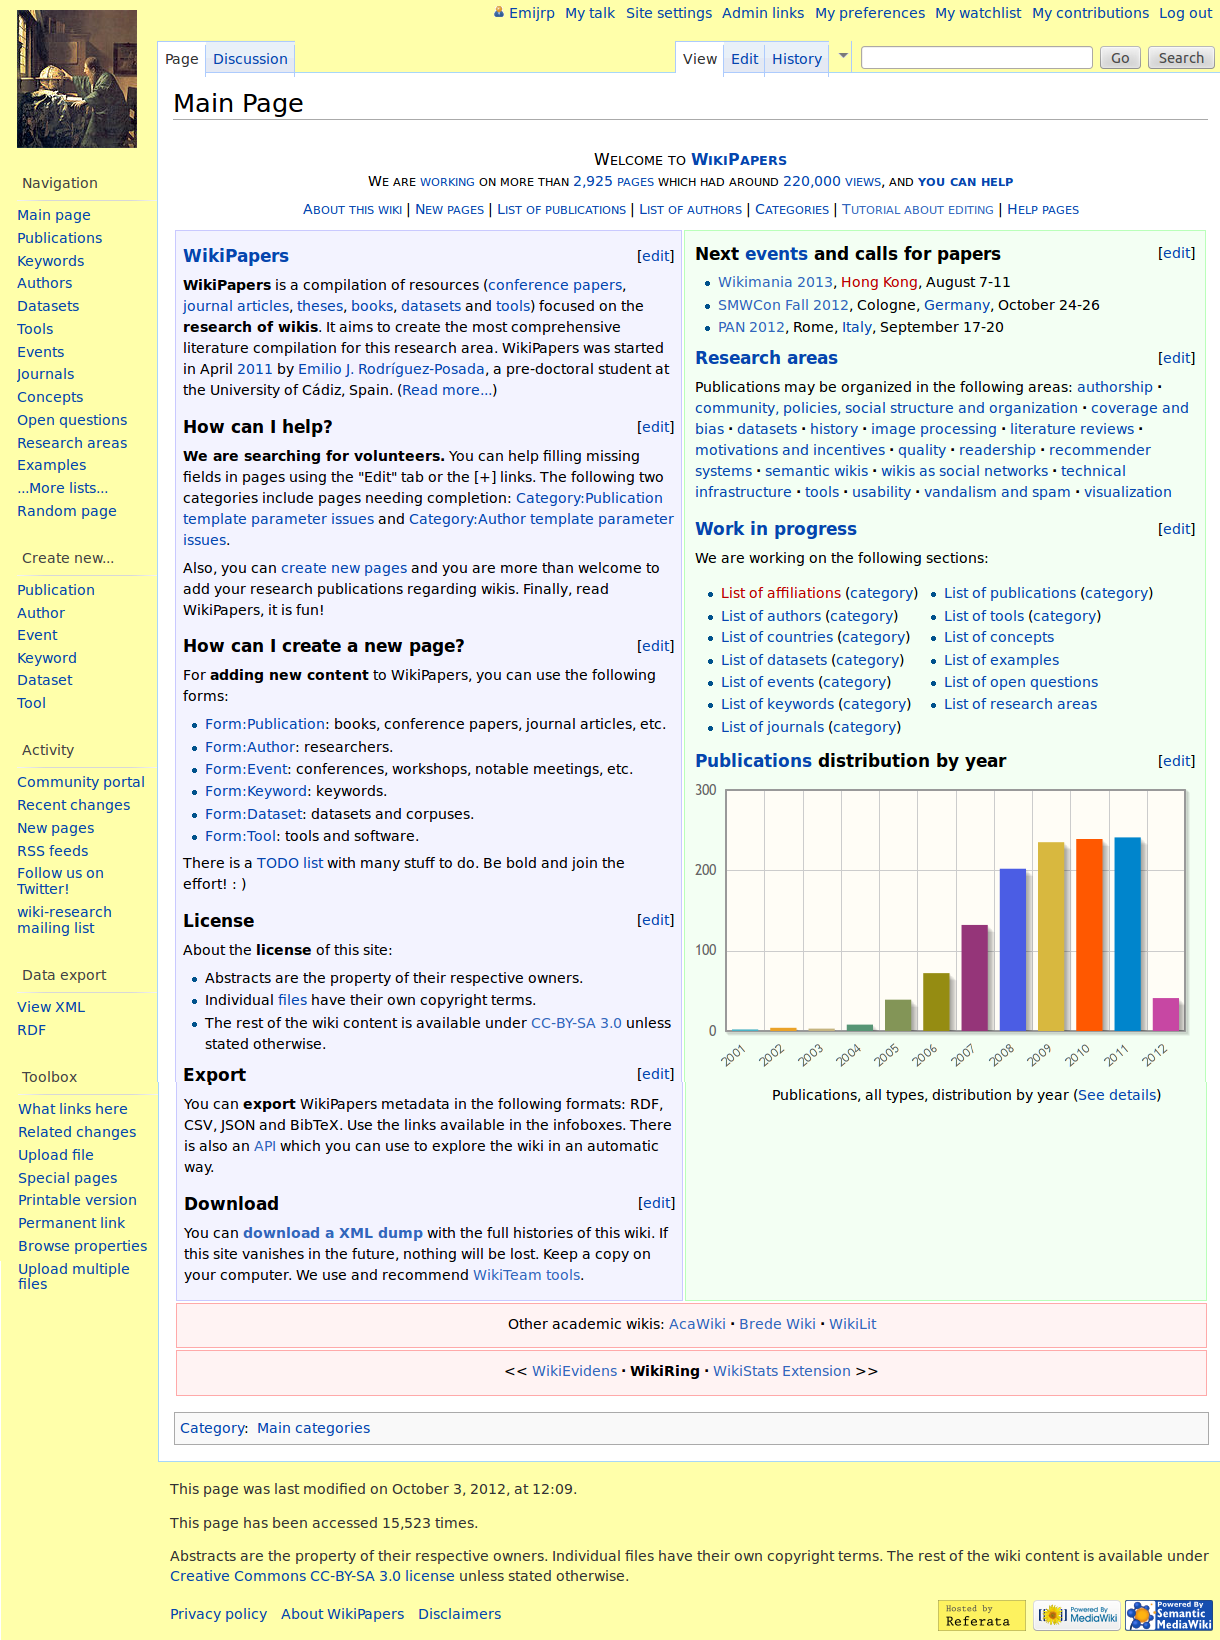
\includegraphics[width=0.9\textwidth]{wpfull.png}
\caption{Portada de WikiPapers.}
\label{fig:wpfull}
\end{figure}

En WikiSym 2011 tuvo lugar un workshop\citep{ayers2011} donde se discutió acerca de qué requisitos debía cumplir un hipotético sistema que recopilara literatura sobre wikis (Tabla~\ref{tab:reqwikisym11}). WikiPapers los cubre en su totalidad.

\begin{table}[htb]
\centering
\begin{tabular}{| c | c |}
\hline
\textbf{Característica} & \textbf{¿Lo ofrece WikiPapers?} \\
\hline
Editable & Sí, es un MediaWiki \\ \hline 
Listas/Grupos & Sí \\ \hline 
Seguimiento/RSS & Sí \\ \hline 
Ver páginas nuevas & Sí, ordenando por fecha \\ \hline 
Categorías/Tags & Sí \\ \hline 
Papers relacionados & Sí \\ \hline 
Referencias/Citas & Sí \\ \hline 
Conferencia/Journal & Sí, tesis y otros \\ \hline 
Peer-reviewed o no & Sí, con un campo \\ \hline 
Importar/Exportar & BibTeX/CSV/RDF/JSON \\ \hline 
Usabilidad & Buena, Semantic Forms \\ \hline 
API & Sí \\ \hline 
Datasets & Sí \\ \hline 
Enlaces & Sí \\ \hline 
Trabajo futuro & Sí, preguntas abiertas \\ \hline 
Free/Libre & Sí, excepto abstracts \\ \hline 
Compatibilidad & RDF/Texto plano \\ \hline 
Licencia de papers & Sí \\ \hline 
Material relacionado & Sí \\ \hline 
Stars/Comentarios & Sí \\ \hline 
No wikitexto & Oculto, Semantic Forms \\ \hline 
\end{tabular}
\caption{Requisitios sugeridos en WikiSym}
\label{tab:reqwikisym11}
\end{table}

\subsection{Publicaciones}
En WikiPapers cada publicación dispone de una página en la que se detallan todos sus metadatos (título, autores, palabras clave, año, revista o congreso, DOI, idioma, licencia, enlaces al fichero y motores de búsqueda), el abstract, las referencias que incluye, las citas que recibe y un espacio de discusión. Los metadatos sirven para hacer búsquedas y filtrar. A noviembre de 2012 ya se dispone de más de 1.700 publicaciones,\footnote{\href{http://wikipapers.referata.com/wiki/List_of_publications}{http://wikipapers.referata.com/wiki/List\_of\_publications}} incluyendo artículos de revistas y congresos, tesis y libros. Todos los metadatos se pueden exportar en los formatos BibTeX, RDF, CSV y JSON.

\subsection{Palabras clave}
Existe un listado de todas las palabras clave\footnote{\href{http://wikipapers.referata.com/wiki/List_of_keywords}{http://wikipapers.referata.com/wiki/List\_of\_keywords}} presentes en los artículos y cada una de ellas cuenta con varios términos relacionados, lo que permite navegar entre ellas. Las más frecuentes son: Wikipedia, wiki, semantic wiki, web 2.0, collaboration, evaluation, collaborative learning, knowledge management, MediaWiki, motivation, data mining y conflict. 

\subsection{Autores}
Para cada autor hay una ficha que incluye su nombre, afiliación, país, índice de coautores, página web, estadísticas sobre número de publicaciones y citas, y por supuesto un listado de publicaciones, \emph{datasets} y herramientas de su creación. Ya están listados unos 1.000 autores (Figura~\ref{fig:autores-tarta}).\footnote{\href{http://wikipapers.referata.com/wiki/List_of_authors}{http://wikipapers.referata.com/wiki/List\_of\_authors}}

\begin{figure}[htb]
\centering
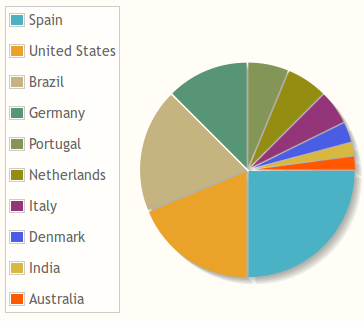
\includegraphics[width=0.6\textwidth]{autores-tarta.png}
\caption{Autores para los que se conoce su nacionalidad.}
\label{fig:autores-tarta}
\end{figure}

\subsection{Datasets}
Un listado de \emph{datasets}\footnote{\href{http://wikipapers.referata.com/wiki/List_of_datasets}{http://wikipapers.referata.com/wiki/List\_of\_datasets}} permite observar la gran cantidad de datos sobre comunidades wiki disponibles para analizar. Existen \emph{datasets} sobre vandalismo, texto wiki enriquecido con semántica, datos extraidos de \emph{infoboxes}, \emph{logs} anonimizados de visitas, mensajes de listas de correo y por supuesto los historiales de Wikipedia.

A este respecto, el proyecto WikiTeam\footnote{\href{http://code.google.com/p/wikiteam/}{http://code.google.com/p/wikiteam/}} está compilando una gran cantidad de datos sobre comunidades wiki, que se cifra ya en 4.500 \emph{dumps}.

\subsection{Herramientas}
Se está construyendo un listado de herramientas\footnote{\href{http://wikipapers.referata.com/wiki/List_of_tools}{http://wikipapers.referata.com/wiki/List\_of\_tools}} que se han desarrollado a la hora de investigar sobre wikis y para proponer soluciones a ciertos problemas.

\subsection{Y más...}
También se está recopilando información sobre revistas, congresos, eventos, conceptos, ejemplos de análisis, preguntas abiertas, encuestas, motores wiki, wikifarms y más. WikiPapers, además de todo lo comentado anteriormente, sirve para que investigadores de wikis hagan comunidad y establezcan conexiones para futuras investigaciones.

\clearpage

\section{Estado del arte}

%Áreas de investigación \href{http://wikipapers.referata.com/wiki/List_of_research_areas}{http://wikipapers.referata.com/wiki/List\_of\_research\_areas}

A continuación presentamos el \textbf{estado del arte} de la investigación sobre wikis haciendo uso de WikiPapers. No incluye todas las publicaciones posibles (está disponible en línea para consultas exhaustivas) pero sí los resultados más importantes hasta ahora, descartando experiencias duplicadas y otras que han quedado desfasadas. WikiPapers dispone actualmente de más de 1700 publicaciones sobre wikis que se han hallado de la siguiente manera:
\begin{itemize}
\item \textbf{Términos de búsqueda:}  wiki, Wikipedia, Wiktionary, Wikibooks, Wikiversity, Wikiquote, Wikisource, Wikinews, Wikispecies, MediaWiki, Wikimedia, wikifarm.
\item \textbf{Zonas de búsqueda:} título, abstract y palabras clave.
\item \textbf{Servicios utilizados:} bases de datos (Scopus), buscadores (Google Scholar), redes sociales (Bibsonomy, CiteULike, CiteSeerX, Zotero) y repositorios de pre-prints (arXiv).
\item \textbf{Fecha:} las búsquedas abarcan desde 2001 hasta 2012.
\end{itemize}

Ha requerido un esfuerzo de eliminación de algunos resultados no relacionados directamente con los wikis. Se escogieron los servicios enumerados por ser los más completos, aunque seguimos en búsqueda de otros y añadiendo las nuevas publicaciones que salen cada mes. En WikiPapers también se han creado páginas para los autores, \emph{datasets} y herramientas relacionadas, a los que también les dedicamos una sección.

Agrupando las publicaciones por categorías temáticas hemos conseguido dividir el estado del arte en las siguientes áreas bien definidas.

\subsection{Autoría y calidad}

%http://wikipapers.referata.com/wiki/List_of_research_areas#Authorship
%http://wikipapers.referata.com/wiki/List_of_research_areas#Quality

La naturaleza abierta de los wikis permite colaborar a todo aquel que lo desee \citep{ward2001}. Se pueden modificar sus contenidos simplemente registrándose en el sitio y muchas veces hasta de forma anónima, como en el caso de Wikipedia. Esto ha llevado a debates, a veces acalorados, sobre la calidad de los contenidos de los wikis.

Wikipedia no se presenta como un ente en posesión de la verdad, sino que expone los distintos puntos de vista\footnote{\href{http://en.wikipedia.org/wiki/Wikipedia:Neutral_point_of_view}{http://en.wikipedia.org/wiki/Wikipedia:Neutral\_point\_of\_view}} sobre cada tema indicando referencias a documentos, libros o webs externas que apoyan cada afirmación, dejando al lector que se forme una opinión contrastada, siempre existiendo la posibilidad de acceder a esas referencias para verificar la información. El proceso de añadir referencias es complejo, desigual en el tiempo y en él no participan todos los usuarios, sino un núcleo más comprometido con cada artículo \citep{chen2012}.

Se han realizado comparaciones de calidad con formas más tradicionales de creación de obras. La más conocida y controvertida es la publicada en \emph{Nature} \citep{giles2005} comparando entradas de Wikipedia con sus homólogas en la \emph{Enciclopedia Britannica}. De 42 artículos analizados sobre ciencia, Wikipedia presentaba cuatro imprecisiones, mientras que \emph{Britannica} tenía tres. Según \emph{Nature}, \emph{Britannica} poseía cierta ventaja sobre Wikipedia pero no tan grande como cabría esperar, al menos en cuanto a artículos científicos. Este estudio provocó que \emph{Britannica} respondiese alegando que \emph{Nature} había cometido errores en el análisis e interpretando sus propios resultados \citep{britannica2006}. \emph{Nature} respondió a las acusaciones de \emph{Britannica}, explicando la metodología y cómo había sido el proceso de revisión de los artículos, y mantuvo que el estudio era correcto \citep{nature2006}.

Análisis como \citep{chesney2006} encontraron errores en un 13\% de los artículos analizados y recogieron que los expertos otorgaban una mayor fiabilidad a los contenidos de Wikipedia mientras que los no expertos recelaban más. Otras comparaciones como \citep{holman2008} encontraron que lo artículos de Wikipedia son fiables en un 80\% frente al 95\%-96\% de sus homólogos en \emph{Enciclopedia Britannica}, \emph{The Dictionary of American History} y \emph{American National Biography Online}.

Los mayoría de motores wiki mantienen los historiales completos desde que una página es creada. Esto permite conocer quién escribió qué y cuándo. Analizando los historiales es posible observar qué oraciones han perdurado más en el tiempo sin ser modificadas. Algunas herramientas, como WikiTrust \citep{adler2008}, usan estos y otros métodos para calcular indicadores de fiabilidad de los textos y lo visualizan con distintos colores por ejemplo. También se está trabajando en clasificadores de artículos por su calidad \citep{wu2012}. Iniciativas como Article Feedback Tool\footnote{\href{http://en.wikipedia.org/wiki/Wikipedia:Article_Feedback_Tool}{http://en.wikipedia.org/wiki/Wikipedia:Article\_Feedback\_Tool}} ayudan a los lectores a evaluar la calidad de los artículos y a informar de errores.

\subsection{Cobertura y sesgos}

%http://wikipapers.referata.com/wiki/List_of_research_areas#Coverage_and_bias

El desarrollo de Wikipedia es muy desigual existiendo problemas de \textbf{cobertura y sesgos} en los contenidos de cada idioma. Actualmente existen versiones de Wikipedia en más de 280 lenguas, siendo la inglesa la que cuenta con mayor número de artículos y usuarios. Wikipedia en inglés es la principal fuente desde la que otras ediciones traducen \citep{warnckewang2012}. La cobertura de temas es diferente y está influenciado por el idioma y la cultura de la que provengan sus usuarios \citep{massa2012}. Temás básicos y fundamentales de arte, historia, geografía, ciencia, tecnología y ocio están presentes en su mayoría pero cuando se trata de biografías o asuntos locales, afloran las diferencias entre los idiomas de la enciclopedia.

%gender

%global south

%minorities

\subsection{Comunidad}

%http://wikipapers.referata.com/wiki/List_of_research_areas#Community.2C_policies.2C_social_structure_and_organization

%vida de los usuarios

\citep{zhang2012}

%caida de la retención de usuarios nuevos

La disminución de la retención de usuarios nuevos en los últimos años se ha achacado a que los recién llegados reciben un «bombardeo» de mensajes cuando actúan de modo incorrecto a las políticas de Wikipedia [REF]. Estos mensajes suelen están ya escritos de antemano para ahorrar tiempo, son extensos, incluyen excesivos enlaces a páginas de normas y resultan muy fríos ya que no parecen escritos por un humano sino procedentes de algún sistema automático de avisos. Experimentos en los que se ha reducido el tamaño del mensaje, el número de enlaces y redactado de manera más informal han arrojado resultados positivos \citep{faulkner2012}.

\subsection{Educación}

%http://wikipapers.referata.com/wiki/List_of_research_areas#Learning.2C_teaching.2C_education

%Wikis como herramientas educativas

%Experiencias docentes

Se han desarrollado infinidad de experiencias docentes empleando wikis propios o wikis públicos como Wikipedia.

\citep{consiglio2012}

\subsection{Datasets}

%http://wikipapers.referata.com/wiki/List_of_research_areas#Datasets
%http://wikipapers.referata.com/wiki/List_of_datasets

Una de las ventajas de la investigación sobre wikis, sobre todo el caso de Wikipedia, es la disponibilidad de \emph{datasets} con los textos completos, historiales, \emph{logs} e información de actividad de los usuarios.

La mayoría de los wikis cuenta con algún tipo de licencia libre, generalmente Creative Commons o GFDL, lo que facilita la adquisición, uso y distribución de los datos, aunque son pocos los que ponen a disposición del público copias completas de las bases de datos. Esto está cambiando a raiz de la aparición de WikiTeam, un proyecto para desarrollar herramientas para preservar wikis, que fundé en 2011 y que ya ha generado datasets para más de 5000 wikis.

Otros datasets sobre wikis que están disponibles se encuentran en la tabla \ref{tab:datasetstable}. Incluyen datos sobre coordenadas de artículos, semántica, páginas borradas, red de enlaces entre páginas, vandalismo, enlaces externos a repositorios, taxonomías y otros.

\href{http://wikipapers.referata.com/wiki/List_of_datasets}{http://wikipapers.referata.com/wiki/List\_of\_datasets}

\begin{sidewaystable}[h]
\centering
\begin{tabular}{| c | c | c | c |}
\hline
\textbf{Dataset} & \textbf{Tamaño} & \textbf{Idioma} & \textbf{Descripción} \\
\hline
CoCoBi & · & Alemán & · \\ \hline 
Coordinates in Wikipedia articles & · & Multilingüe & · \\ \hline 
DBpedia & · & Multilingüe & · \\ \hline 
DeletionPedia & · & Inglés & · \\ \hline 
Domas visits logs & · & Multilingüe & · \\ \hline 
Google dataset linking strings and concepts & · & Multilingüe & · \\ \hline 
PAN Wikipedia vandalism corpus 2010 & · & Inglés & · \\ \hline 
PAN Wikipedia vandalism corpus 2011 & · & Multilingüe & · \\ \hline 
PlusPedia & · & Alemán & · \\ \hline 
Repos-2012-dataset & · & Multilingüe & · \\ \hline 
Social networks of Wikipedia dataset & · & · & · \\ \hline 
WikiBiography & · & · & · \\ \hline 
WikiCorpus & · & Multilingüe & · \\ \hline 
WikiIndex & · & Inglés & · \\ \hline 
WikiNet & · & Multilingüe & · \\ \hline 
WikiPapers & · & Inglés & · \\ \hline 
WikiRelations & · & Inglés & · \\ \hline 
WikiTaxonomy & · & · & · \\ \hline 
WikiTeam dumps & · & Multilingüe & · \\ \hline 
Wikia dumps & · & Multilingüe & · \\ \hline 
Wikimedia dumps & · & Multilingüe & · \\ \hline 
Wikipedia Historical Attributes Data & · & Inglés & · \\ \hline 
Wikipedia Vandalism Corpus (West) & · & Inglés & · \\ \hline 
Wikipedia page-to-page link database & · & Inglés & · \\ \hline 
WikipediaXML & · & Multilingüe & · \\ \hline 
Wlm-2011-dataset & · & Multilingüe & · \\ \hline
\end{tabular}
\caption{Datasets relacionados con wikis.}
\label{tab:datasetstable}
\end{sidewaystable}

\subsection{GLAM}

%http://wikipapers.referata.com/wiki/List_of_research_areas#GLAM

Las Galerías, Bibliotecas, Archivos y Museos (conocido como GLAM) dedican mucho presupuesto a digitalizar material y a ponerlo a disposición del público en Internet. Análisis de los enlaces existentes hacia bibliotecas y archivos digitales de patrimonio cultural, realizados sobre Wikipedia en español y catalán, han mostrado que el número de referencias de este tipo es muy bajo aún para la mayoría de las colecciones, exceptuando algunas muy conocidas como la Biblioteca Virtual Miguel de Cervantes\citep{saorin2012}.

La mayoría de estas instituciones han comprendido la importancia de que sitios tan visibles como Wikipedia, bien posicionados en buscadores como Google, incluyan enlaces a sus colecciones digitalizadas, para aumentar su tráfico y difusión \citep{lally2007, elder2012}. Tal es así que, por ejemplo, Europeana ha incluido un widget «citar en Wikipedia» para que sus contenidos sean fácilmente enlazables desde la enciclopedia libre. No se trata en exclusiva de dotar de visibilidad a estas colecciones digitales añadiendo estos enlaces a Wikipedia, sino de aumentar la calidad de los artículos de la enciclopedia, apoyando las afirmaciones que se hacen en los textos, los cuales muchos de ellos muestran deficiencias o son referenciados con material poco académico \citep{nielsen2007, luyt2010}.

%WLM 2011

Más cercano a la conservación y difusión del patrimonio monumental de los países se encuentra Wiki Loves Monuments. Esta iniciativa fue creada en 2010 con la intención de fotografiar monumentos para poder ilustrar los artículos de Wikipedia. La primera edición se realizó exclusivamente en los Países Bajos, en 2011 se extendió a 18 países europeos y en 2012 a otros países del mundo \citep{rodriguez2012wlm}.

%Wiki Loves Libraries

%Wikipedian in Residence

Para establecer vínculos entre la comunidad de editores de Wikipedia y estas instituciones culturales se ha creado la figura del «Wikipedian in Residence».\footnote{\href{http://outreach.wikimedia.org/wiki/Wikipedian_in_Residence}{http://outreach.wikimedia.org/wiki/Wikipedian\_in\_Residence}}. El wikipedista trabaja durante unos meses con la organización ayudándole a comprender las dinámicas de la enciclopedia libre, fomentando el desarrollo de los artículos que traten sobre las colecciones de la institución, organizando eventos o visitas donde se aprenda a participar en Wikipedia, entre otras posibles tareas como la coordinación en la liberación de material digitalizado bajo licencias libres compatibles con Wikipedia. Es una iniciativa que ha tenido bastante éxito y muchas instituciones culturales de todo el mundo se están acogiendo a ella con interés, por ejemplo el British Museum, Museu Picasso o Smithsonian Institution Archives.


\subsection{Herramientas}

%http://wikipapers.referata.com/wiki/List_of_research_areas#Tools
%http://wikipapers.referata.com/wiki/List_of_tools

Entorno a los wikis se generado un espectro de herramientas específicas. Unas (Figura~\ref{tab:vandaltoolstable}) ayudan a detectar, reparar y eliminar vandalismos y ataques de spam, uno de los pocos inconvenientes que tienen los wikis al ser sistemas tan abiertos a la colaboración. Otras herramientas, más enfocadas a la investigación, facilitan el acceso a los datos de los wikis (Figura~\ref{tab:frameworkstable}), a procesarlos (Figura~\ref{tab:dataprocessingtoolstable}) y visualizarlos (Figura~\ref{tab:visualizationtoolstable}).

\href{http://wikipapers.referata.com/wiki/List_of_tools}{http://wikipapers.referata.com/wiki/List\_of\_tools}

\begin{sidewaystable}[h]
\centering
\begin{tabular}{| c | c | c | c | c |}
\hline
\textbf{Herramienta} & \textbf{S.O.} & \textbf{Idioma} & \textbf{Licencia} & \textbf{Descripción} \\
\hline
AVBOT & Multiplataforma & Español & GPL & Bot anti-vandalismo para Wikipedia en español. \\ \hline
ClueBot & GNU/Linux & · & · & · \\ \hline
CryptoDerk's Vandal Fighter & Multiplataforma & Inglés & · & · \\ \hline
Huggle & Windows & · & GPL & · \\ \hline
Igloo & · & · & · & · \\ \hline
STiki & Multiplataforma & Inglés & GPL & · \\ \hline
Salebot & · & · & · & · \\ \hline
Twinkle & · & · & · & · \\ \hline
Vandal Fighter & Multiplataforma & Inglés & · & · \\ \hline
VandalProof & Windows & Inglés & · & · \\ \hline
VandalSniper & Multiplataforma & Inglés & · & · \\ \hline
\end{tabular}
\caption{Herramientas anti-vandalismo y anti-spam.}
\label{tab:vandaltoolstable}
\end{sidewaystable}


\begin{sidewaystable}[h]
\centering
\begin{tabular}{| c | c | c | c | c |}
\hline
\textbf{Herramienta} & \textbf{S.O.} & \textbf{Idioma} & \textbf{Licencia} & \textbf{Descripción} \\
\hline
Java Wikipedia Library & Multiplataforma & Inglés & LGPL & Framework en Java. \\ \hline
Perlwikipedia & Multiplataforma & Inglés & GPL & Framework en Perl. \\ \hline
Python-wikitools & Multiplataforma & Inglés & GPL & Framework en Python. \\ \hline
Pywikipediabot & Multiplataforma & Inglés & MIT license & Frame work en Python. El más usado. \\ \hline
\end{tabular}
\caption{Frameworks.}
\label{tab:frameworkstable}
\end{sidewaystable}


\begin{sidewaystable}[h]
\centering
\begin{tabular}{| c | c | c | c | c |}
\hline
\textbf{Herramienta} & \textbf{S.O.} & \textbf{Idioma} & \textbf{Licencia} & \textbf{Descripción} \\
\hline
JWordNet-Similarity & Multiplataforma & Inglés & · & · \\ \hline 
Manypedia.com & Multiplataforma & Inglés & Affero GPL & · \\ \hline 
Wikokit & Multiplataforma & Inglés & Varias & · \\ \hline 
Zawilinski & Multiplataforma & · & · & · \\ \hline 
\end{tabular}
\caption{Herramientas sobre el lenguaje.}
\label{tab:languagetoolstable}
\end{sidewaystable}


\begin{sidewaystable}[h]
\centering
\begin{tabular}{| c | c | c | c | c |}
\hline
\textbf{Herramienta} & \textbf{S.O.} & \textbf{Idioma} & \textbf{Licencia} & \textbf{Descripción} \\
\hline
DiffDB & · & · & · & · \\ \hline 
Ikiwiki & · & · & · & · \\ \hline 
Infobox2rdf & · & · & · & · \\ \hline 
MediaWiki API & · & · & · & · \\ \hline 
Sioc MediaWiki & · & · & · & · \\ \hline 
Wiki Edit History Analyzer & · & · & · & · \\ \hline 
Wiki2XML parser & · & · & · & · \\ \hline 
WikiPrep & · & · & · & · \\ \hline 
Wikihadoop & · & · & · & · \\ \hline 
Wikimedia Utilities & · & · & · & · \\ \hline 
Wikipedia Extractor & · & · & · & · \\ \hline 
Wikipedia Miner & · & · & · & · \\ \hline 
Wikipedia-map-reduce & · & · & · & · \\ \hline 
\end{tabular}
\caption{Herramientas de procesamiento de datos.}
\label{tab:dataprocessingtoolstable}
\end{sidewaystable}


\begin{sidewaystable}[h]
\centering
\begin{tabular}{| c | c | c | c | c |}
\hline
\textbf{Herramienta} & \textbf{S.O.} & \textbf{Idioma} & \textbf{Licencia} & \textbf{Descripción} \\
\hline
HistoryFlow & · & · & · & · \\ \hline 
StatMediaWiki & · & · & · & · \\ \hline 
Wiki Explorator & · & · & · & · \\ \hline 
Wiki Trip & · & · & · & · \\ \hline 
WikiBlame & · & · & · & · \\ \hline 
WikiChanges & · & · & · & · \\ \hline 
WikiEvidens & · & · & · & · \\ \hline 
WikiPride & · & · & · & · \\ \hline 
WikiScanner & · & · & · & · \\ \hline 
WikiTracer & · & · & · & · \\ \hline 
WikiTrust & · & · & · & · \\ \hline 
WikiVis (FH-KL) & · & · & · & · \\ \hline 
WikiVis (UM) & · & · & · & · \\ \hline 
WikiWarMonitor & · & · & · & · \\ \hline 
WikiXRay & · & · & · & · \\ \hline 
Wikistream & · & · & · & · \\ \hline 
Wmcharts & · & · & · & · \\ \hline 
\end{tabular}
\caption{Herramientas de visualización.}
\label{tab:visualizationtoolstable}
\end{sidewaystable}


\begin{sidewaystable}[h]
\centering
\begin{tabular}{| c | c | c | c | c |}
\hline
\textbf{Herramienta} & \textbf{S.O.} & \textbf{Idioma} & \textbf{Licencia} & \textbf{Descripción} \\
\hline
WikiSim & · & · & · & · \\ \hline 
WikiTeam tools & · & · & · & · \\ \hline 
· & · & · & · & · \\ \hline 
\end{tabular}
\caption{Otras herramientas.}
\label{tab:othertoolstable}
\end{sidewaystable}


\subsection{Infraestructura}

%http://wikipapers.referata.com/wiki/List_of_research_areas#Technical_infrastructure

%por ejemplo los wikis al estilo p2p para repartir la carga... había una tesis sobre eso en danés?


\subsection{Motivaciones e incentivos}

%http://wikipapers.referata.com/wiki/List_of_research_areas#Motivations_and_incentives

%Encuestas...

\subsection{Motores wiki}

Aunque MediaWiki sea el motor wiki más conocido y utilizado, hay muchos otros. La existencia de tantos motores dificulta la interoperabilidad entre ellos y existen intentos de unificar o al menos promover una sintaxis estándar, como el proyecto WikiCreole\footnote{\href{http://www.wikicreole.org}{http://www.wikicreole.org}}.

Existe un portal que enumera a la mayoría de ellos, llamado WikiMatrix\footnote{\href{http://www.wikimatrix.org}{http://www.wikimatrix.org}}. Contiene información acerca de más de 125 motores wiki y permite hacer comparaciones sobre la presencia o carencia de funcionalidades. Las características se organizan en las siguientes categorías: generales, requisitos del sistema, almacenamiento, seguridad y anti-spam, desarrollo y soporte, funcionalidades comunes y especiales, tipos de enlaces permitidos, sintaxis, usabilidad, estadísticas, formatos de salida, ficheros permitidos y funciones extra.

\subsection{Predicción y tendencias}

Wikipedia se ha constituido como una fuente de consulta de primer orden. Cuando ocurre algún suceso de gran envergadura (desastres, eventos deportivos, fallecimientos de famosos) inmediatamente se ve reflejado en el número de visitas y ediciones a los artículos relacionados.

Se han desarrollado sistemas que detectan esta tendencias y evaluan las subidas repentinas de actividad, mostrando los artículos que más interés han atraido en las últimas horas o días \citep{osborne2012}. También herramientas que evaluando las preferencias de los usuarios, les muestran aquellos temas candentes \citep{ciglan2010}.

%http://wikipapers.referata.com/wiki/Seeking_health_information_online:_does_Wikipedia_matter%3F

La magnitud de Wikipedia, la rapidez de actualización de sus contenidos y la gran cobertura que tiene para la práctica totalidad de temas de relevancia, la hacen una fuente de conocimiento estructurado de gran valor. Se están desarrollando algunos experimentos para utilizarla para predicciones, por ejemplo para preveer recaudaciones en taquilla \citep{mestyan2012}. Otros ejemplos incluyen el intento de intuir movimientos en los mercados financieros a través de Wikipedia.\footnote{\href{http://rb.imm.dtu.dk/base/c/}{http://rb.imm.dtu.dk/base/c/} y \href{http://rb.imm.dtu.dk/base/c/Lundbeck}{http://rb.imm.dtu.dk/base/c/Lundbeck}}

\subsection{Preservación}

Existe claramente un antes y un después en la generación y publicación de contenidos en Internet desde la invención del primer software wiki y de la creación de Wikipedia en 2001. Todo este contenido producido por millones de usuarios distribuidos por todo el planeta necesita ser preservado, no solo por su valor en conocimiento sino también por formar parte ya de la historia de Internet.

Proyectos wiki grandes y muy comprometidos con el conocimiento libre como Wikipedia publican copias de seguridad de todos sus artículos e historiales completos. Esto facilita la difusión y preservación para la posteridad. En cambio otros proyectos wiki más reducidos, pero muy numerosos, no tienen por costumbre publicar copias para descarga de sus contenidos.

Preservar los historiales completos y otros metadatos de los wikis no es una tarea trivial y plantea algunas dificultades. Por ello ciertas herramientas o servicios como Internet Archive o WebCitation no funcionan bien en estos casos. Curiosamente no ha habido mucho esfuerzo por cambiar la situación en este tema hasta hace relativamente poco tiempo.

%urobe
\citep{popitsch2010} propusieron un sistema para preservar los contenidos y metadatos de wikis que usaran distintos motores, de modo que también buscaban crear una sintaxis común. El proyecto quedo suspendido por falta de fondos.

%revisar el paper de wikiteam

Al año siguiente se creó WikiTeam\footnote{\href{http://code.google.com/p/wikiteam/}{http://code.google.com/p/wikiteam/}}, un grupo de voluntarios que desarrolla herramientas de preservación para wikis. Hasta el momento funcionan únicamente sobre MediaWiki pero ya han logrado preservar más de 4.500 wikis de toda la red.

\subsection{Procesamiento de imágenes}

%Poquísimo hay hecho me parece a mí...

\subsection{Procesamiento del lenguaje natural}

%wiktionary

\subsection{Recomendación de tareas}

La \textbf{recomendación de tareas} es un área todavía por explorar y explotar en los wikis. Dado que las comunidades wiki funcionan colaborando, los usuarios deben conocer qué artículos requieren su intervención para mejorar o ampliar los contenidos, subir imágenes, corregir errores, etc. Esta es una tarea que se hace de forma manual principalmente. El usuario recorre el wiki, leyendo sus contenidos, y descubre por azar páginas o secciones que necesitan ayuda. Hasta el momento existen muy pocas experiencias que hayan intentado resolver este asunto de forma automática.

%había un bot en la inglesa también no?


%Images for bio
Una de ellas es \emph{Images for biographies}\footnote{\href{http://toolserver.org/~emijrp/imagesforbio/}{http://toolserver.org/~emijrp/imagesforbio/}}, una aplicación web que muestra imágenes que pueden servir para las biografías de Wikipedia. Comparando las imágenes que se usan en otros idiomas de Wikipedia, recomienda esas imágenes para la misma biografía en otro idioma, si es que carece de fotografía. Este sistema ha ayudado a ilustrar miles de páginas y además es bastante sencillo de utilizar.

%reporte de errores

La gestión de errores en los artículos de Wikipedia siempre se había hecho utilizando las páginas de discusión adjuntas. En ellas la gente comenta los problemas que observan y se resuelven de manera conjunta. Estas páginas de informe de fallos pasan desapercibidas para los que son meros lectores de los artículos y no wikipedistas. Para implicar más a este sector de usuarios pasivos se han desarrollado algunos experimentos, por ejemplo Article Feedback Tool\footnote{\href{http://en.wikipedia.org/wiki/Wikipedia:Article_Feedback_Tool}{http://en.wikipedia.org/wiki/Wikipedia:Article\_Feedback\_Tool}}, para facilitar el avisar de fallos. Es un trabajo en proceso pero está dando buenos resultados, ya que agiliza el informe y reparación de errores en los artículos.

%detección de temas controversiales con reversiones

Finalmente, se han desarrollado algunas metodologías y algoritmos para detectar artículos controversiales en base a cómo interactúan entre sí los usuarios que los redactan \citep{sepehrirad2012}. Esto puede ayudar a encontrar páginas que requieran la participación de usuarios adicionales para resolver las disputas en los contenidos.

\subsection{Semántica}

%semantic mediawiki, ventajas, inconvenientes

El motor MediaWiki dispone de una extensión semántica llamada Semantic MediaWiki...

%referata

%SWEETpedia

\subsection{Usabilidad}

%mejoras históricas de la usabilidad de MediaWiki

%intentos por mejorar la usabilidad para atraer más usuarios

%

\subsection{Vandalismo y spam}

%http://wikipapers.referata.com/wiki/Vandalism
%http://wikipapers.referata.com/wiki/List_of_anti-vandalism_tools
%http://wikipapers.referata.com/wiki/List_of_vandalism_datasets

El caracter abierto de los wikis, en los que cualquiera puede modificar los contenidos, facilita la rápida mejora de los textos pero también que usuarios malintencionados o robots puedan causar destrozos, comúnmente llamados vandalismos, o añadir spam.

Se han empleado diferentes enfoques para contrarestar estos efectos negativos. Se pueden clasificar en las siguientes categorías:
\begin{enumerate}
\item \textbf{Páginas de control de cambios:} se puede considerar el control más básico de todos, saber qué páginas han sido modificadas en los últimos instantes. Ejemplos: la página de «Cambios recientes».
\item \textbf{Herramientas semiautomáticas:} resaltan cambios que pueden ser dañinos, pero requieren intervención humana para decidir si revertir o no. Ejemplos: AbuseFilter, Huggle, STiki.
\item \textbf{Permisos de edición por grupo de usuarios:} en función de a qué grupo perteneza un usuario, podrá o tendrá vetada la modificación de ciertas páginas. Ejemplos: semiprotección y protección de páginas.
\item \textbf{Herramientas automáticas:} conocidas como bots anti-vandalismo. Existen bots especializados en mero vandalismo o en spam. Ejemplos: AVBOT, ClueBot, Salebot.
\item \textbf{Aprobación de cambios:} herramientas que acumulan los cambios y no los hace visibles hasta que alguien los aprueba. Ejemplos: FlaggedRevisions.
\item \textbf{Catpchas:} paran el spam antes de que se produzca, no quedando registrado en los historiales. Ejemplo: captcha de preguntas, reCAPTCHA.
\item \textbf{Soluciones específicas:} cuando hay muchas ediciones de un mismo usuario que revertir o muchas páginas que borrar debido a un ataque. Ejemplo: Rollbacker, la extensión Nuke.
\end{enumerate}

Obviamente, las soluciones que requiere intervención humana son herramientas con nula o escasa «inteligencia» o algoritmia. Donde se ha desarrollado una mayor labor investigadora, aunque aun limitada, es en el desarrollo de herramientas automáticas que recorren los cambios recientes del wiki y revierten de manera autónoma cuando detectan un cambio dañino. Ejemplos de estos sistemas que llevan funcionando algunos años incluyen AVBOT \citep{avbot2009, avbot2010} en Wikipedia en español y ClueBot \citep{carter2008} en Wikipedia en inglés.

%PAN/CLEF
CLEF/PAN Lab es un congreso que ha centrado algunas de sus ediciones en la detección de vandalismos en wikis. Publicando un dataset con modificaciones marcadas como vandalismo y otras como benignas, invitaba a desarrollar algoritmos que aprendiendo de estos casos de entreamiento, fueran capaces de detectar futuros casos de vandalismo.

%comentar un poco que características se han demostrado más útiles para detectar vandalismo

%datasets de vandalismo
El entrenamiento de algoritmos se basa como hemos comentado en datasets que contienen casos positivos y negativos. Lo que sucede es que es necesario que un humano haga esta categorización de antemano. Existe interés en desarrollar datasets utilizando los historiales de Wikipedia como fuente de casos positivos y negativos, a partir de las reversiones que hacen humanos \citep{west2010}.

\subsection{Visualización}

%http://wikipapers.referata.com/wiki/List_of_visualization_tools

La gran cantidad de datos disponible sobre wikis públicamente, además de que sus licencias permiten la libre reutilización, hacen necesaria y posible la aparición de numerosas herramientas de \textbf{visualización} que ayudan a entender cómo funcionan estas comunidades.

Desde los primeros años de Wikipedia se han creado herramientas y servicios para poder visualizar y comprender la evolución del proyecto. Desde tablas y gráficas sencillas sobre número de páginas, usuarios o ediciones por unidad de tiempo, hasta ranking de páginas según el nivel de actividad o mapas. Las estadísticas oficiales de Wikipedia se encuentran en \href{http://stats.wikimedia.org}{stats.wikimedia.org} y una recopilación con algunos ejemplos muy llamativos también está disponible.\footnote{\href{http://infodisiac.com/Wikimedia/Visualizations/}{http://infodisiac.com/Wikimedia/Visualizations/}}

%comentar las herramientas de visualización que hay (aunque ya están en la tabla)...

%HistoryFlow
Entre las herramientas de visualización con mayor éxito en su momento fue HistoryFlow \citep{viegas2004}, que permite observar la evolución de un documento (en este caso una página cualquiera de Wikipedia) que haya sido redactado entre varios autores. Esto facilita ver qué partes de texto han perdurado en el tiempo, quién ha escrito qué oraciones, número de aportaciones, etc.

%StatMediaWiki
Para wikis con pocos usuarios y páginas StatMediaWiki\footnote{\href{http://statmediawiki.forja.rediris.es}{http://statmediawiki.forja.rediris.es}} ofrece una gran cantidad de análisis. Mediante tablas y gráficas muestra la actividad por usuario, página y grupos de páginas. Se ha utilizado para evaluar el trabajo de alumnos en wikis de asignaturas universitarias \citep{rodriguez2011, palomoile2012, palomorevision2012, palomorusc2012}.

%Wikistream
Para poder observar cuál es el ritmo de actividad de Wikipedia existen diversas herramientas, pero Wikistream\footnote{\href{http://wikistream.inkdroid.org}{http://wikistream.inkdroid.org}} es una que comple muy bien su cometido. Permite filtrar las modificaciones de usuarios registrados, anónimos y bots, también por idioma y espacio de nombres.

%Wmcharts
%Wiki Trip
%WikiVis
%WikiViz

Existen muchas otras como wmcharts, WikiTrip, WikiVis, Wikitweets, etc. Cada año que pasa están disponibles nuevos conjuntos de datos y los que había con anterioridad crecen en tamaño. En 2011 tuvo lugar WikiViz, una competición que premiaba a los mejores trabajos que lograran visualizar el impacto de Wikipedia en la sociedad, lo que muestra el gran interés que hay en este sentido.

\subsection{Wikifarms}

%http://wikipapers.referata.com/wiki/List_of_research_areas#Wiki_engines

El concepto wiki, como sitio web que permite a los usuarios consultar y modificar sus contenidos, lo creó Ward Cunningham en 1996. En 2001 se fundó Wikipedia y desde entonces esta forma de generar contenido colaborativamente se ha popularizado. El motor wiki más utilizado es MediaWiki, pero existen muchos más, entorno a los 100, la mayoría de ellos muy desconocidos.

Los usuarios de Wikipedia pronto se dieron cuenta de que, debido a las políticas de notabilidad y verificabilildad, había muchos contenidos que pudiéndose aprovechar del sistema wiki, no tenían cabida en la enciclopedia libre. Dado que MediaWiki es software libre, pronto aparecieron otros sitios web que haciendo uso de este motor, animaba a sus usuarios a generar contenido colaborativamente sobre los temas más variopintos.

Un paso más se dio cuando aparecieron las conocidas como \textbf{wikifarms} que no son más que \emph{hostings} que facilitan al usuario la creación de sitios similares a Wikipedia, aislándote de todo el proceso de instalación en el servidor de las herramientas. En una wikifarm, con solo registrarte, dispones de un wiki listo para volcar material y mejorarlo con una comunidad.

Entre las wikifarms más conocidas se encuentra Wikia, pero existen otras como EditThis, ShoutWiki, TropicalWikis y Wikkii. También existe una especializada en wikis semánticos, Referata.

Uno de los inconvenientes de usar una wikifarm es que normalmente no se tiene acceso directo a la base de datos donde se almacenan todos los contenidos o al directorio donde se guardan las imágenes subidas. Esto supone, para el usuario externo, graves dificultades a la hora de hacer una copia de seguridad del wiki en cuanto tiene unos cientos de páginas e imágenes, ya que hace impracticable el guardar local y manualmente una copia de cada página.

Existen casos de wikifarms que han tenido problemas en el servidor, y dada la ausencia de copias de seguridad en el mismo y a la imposibilidad práctica de que los usuarios la hicieran para ellos mismos, han perdido todos los datos. En 2011 se fundó un proyecto llamado WikiTeam que ha desarrollado herramientas que recorren un wiki dado y descarga todos los contenidos, historiales e imágenes. Esta solución supone un gran avance en cuanto a la preservación de contenido wiki en Internet y reduce las inseguridades a la hora de utilizar una wikifarm para un proyecto propio.

En cuanto a la investigación de wikifarms, existe muy poco trabajo hecho hasta el momento. \citep{kittur2010} hizo un análisis de 6000 wikis de Wikia, pero es poco frecuente ver estudios sobre otros wikis distintos a Wikipedia, cosa que debería ir cambiando con el tiempo si realmente se quiere tener una visión completa y no sesgada a la hora de analizar comunidades wiki de Internet.

\subsection{Wikis como redes sociales}

%http://wikipapers.referata.com/wiki/List_of_research_areas#Wikis_as_social_networks

\clearpage

\section{Cuestiones abiertas}

%http://wikipapers.referata.com/wiki/List_of_open_questions

Es cierto que algunas áreas en el campo de los wikis han sido muy prolíficas en cuanto a publicaciones, pero aun quedan muchas \textbf{cuestiones abiertas}, incluso algunos temas están mínimamente explorados.

%Recommender systems for users: tools that offer tasks to do based on mining past user edits.

Uno muy poco desarrollado y que podría tener un efecto muy positivo es el de los \textbf{sistemas de recomendación}. Fabricar sistemas que indiquen a los usuarios dónde es necesaria su intervención en función de sus preferencias sería muy beneficioso. Por ejemplo, en el contexto de Wikipedia, automatizar la petición de imágenes para artículos sobre municipios o monumentos según la localización del usuario o sugerir artículos a mejorar que estén relacionadas con los temas que el usuario lee o edita con frecuencia. O también detectar temas que falten, utilizando otras Wikipedias como fuente, ya que el desarrollo de las enciclopedias en distintos idiomas es desigual, excepto en temas básicos, ya que lo que exista en una no tiene porqué existir en otras más lejanas (por diferencias culturales). Esto ayudaría a optimizar la participación y a eliminar la falsa sensación de que «en Wikipedia está casi todo hecho ya».

%Computer Vision to categorize Wikimedia Commons images (example of Python code, it requires [1])

Otra cuestión a explorar es el \textbf{análisis de imágenes}. Wikimedia Commons es una mediateca libre con más de 12 millones de imágenes y su mantenimiento es muy costoso de hacer manualmente. Herramientas que pudieran ayudar a organizar las imágenes reconociendo objetos o características destacables liberarían de bastante trabajo a los miembros del proyecto.

%What is the community size of wikisphere wikis? [2] (a dataset of wikisphere wikis basic parameters?)
%Research on Wikipedia sister projects: little is known.
%Research on Wikipedias other than English one.
%Research on other wiki communities and wikifarms. 

Un asunto importante es que la inmensa mayoría de publicaciones hablan exclusivamente de Wikipedia y más concreatemente de la versión inglesa, \textbf{ignorando sus proyectos hermanos u otros idiomas}. El segundo proyecto wiki más estudiado es Wiktionary, pero otros como Wikiversidad, Wikilibros o Wikinoticias han atraido escasa o nula atención. Y no solo eso, sino también \textbf{se obvian las miles de comunidades wiki} existentes en la red. No se reproducen los estudios o experiencias en estos otros lugares, donde quizás puedan salir resultados distintos o corroborarlos. Es cierto que hasta hace poco no era sencillo hacerse con una copia completa de las páginas, historiales y metadatos de la mayoría de los wikis de Internet para analizarlos, a menos que el administrador colaborara proporcionándola. Con WikiTeam esto está cambiando, ya que sus herramientas extraen todos los datos de manera sistemática sin necesidad de intervención de los administradores de cada wiki, lo que abre nuevas posibilidades.

%vandalismo
En cuanto al estudio de \textbf{algoritmos para luchar contra el vandalismo}, si bien se han hecho avances y ha habido congresos sobre el tema, distan de tener una precisión adecuada para funcionar de manera autónoma, a menos que se restrinja mucho su actuación solo a los casos de vandalismo o spam más flagrantes. Aun queda mucho por mejorar en este sentido.

Para finalizar, recientemente se ha creado \textbf{Wikidata}, un nuevo proyecto hermano de Wikipedia que recopilará una ingente cantidad de datos de forma estructurada que luego serán utilizados en Wikipedia y otros proyectos. Es muy posible que genere interés entre los investigadores en cuanto adquiera algo de tamaño, como sucedió en el pasado con la enciclopedia libre.

\clearpage

\section{Conclusiones y trabajo futuro}

%porqué hacía falta WikiPapers

En este proyecto de investigación hemos analizado los distintos enfoques utilizados hasta ahora para recopilar literatura sobre wikis. Tras evaluar sus ventajas e inconvenientes, procedimos a desarrollar un sistema, que solucionara las deficiencias conservando lo que se ha comprobado que funciona bien en otros casos y añadiendo las sugerencias que investigadores habían comentado en distintos foros. Entre las características fundamentales de este nuevo enfoque se encuentran: permite participar en la recopilación de literatura de manera colaborativa, aprovecha los metadatos para convertirlos en propiedades de la web semántica (relaciona conceptos, permite consultas, infiere conocimiento), facilita la continua actualización y puesta al día de los contenidos evitando quedar desactualizado como los Systematic Literature Review típicos y hace trivial la exportación y reutilización de los datos, entre otros.

%lo que se ha hecho, cifras, resumen del estado del arte: áreas, alguna curiosidad...

El proyecto resultante ha sido WikiPapers, un wiki para recopilar literatura sobre wikis e información sobre \emph{datasets} y herramientas relacionadas. Hasta el momento se han añadido metadatos para más de 1700 publicaciones, 50 datasets y casi 100 herramientas. La literatura sobre wikis se ha clasificado en las siguientes categorías: autoría y calidad, cobertura y segos, comunidad, educación, datasets, GLAM, herramientas, infraestructura, motivaciones e incentivos, motores wiki, predicción y tendencias, preservación, procesamiento de imágenes, procesamiento del lenguaje natural, recomendación de tareas, semántica, usabilidad, vandalismo y spam, visualización, wikifarms y wikis como redes sociales. El estado del arte planteado en este trabajo sigue esta organización.

%lo que queda por hacer y como ayudar
Aunque WikiPapers ya ha conseguido recopilar una gran parte de la literatura sobre wikis, aun es posible mejorar la cobertura y seguir añadiendo las últimas publicaciones que vayan saliendo. Para esto es necesario conformar una comunidad comprometida con el proyecto. Varios investigadores de wikis ya han mostrado interés y participado, incluyendo sus publicaciones o las de sus colegas. También ha habido colaboraciones anónimas.

%el futuro y más allá...


\clearpage

\bibliographystyle{wink}        
\bibliography{proyecto-investigacion-2012}

%wikisym2012 por encajar
%\citep{schneider2012} Deletion Discussions in Wikipedia: Decision Factors and Outcomes
%\citep{westweber2012} Drawing a Data-Driven Portrait of Wikipedia Editors
%
%

\section*{Licencia}
Esta obra está bajo licencia \href{http://creativecommons.org/licenses/by-sa/3.0/}{Creative Commons Reconocimiento-CompartirIgual 3.0 Unported}.

\end{document}
